\chapter{\viztomotitle: visualization of the \drexmtitle{} output} 
\label{chapter:viztomo}

\viztomotitle{} is a software that includes routines for post-processing the \cijkltitle{} output files generated with \drexmtitle{} and for visualizing the elastic tensor \textbf{C} and left stretch tensor \textbf{FSE} with \paraviewtitle{}. The software also allows computing extrinsic elastic anisotropy (which can or not be superimposed over the LPO fabrics) and provides grid structured distributions of elastic tensors for seismological model simulations.\\
\\
\texttt{COMPILE: ./bash\_compile}\\*
\\
\texttt{RUN: ./viztomo viztomo\_input.dat}\\*

\section{Parameter input file}

The parameter input file is \texttt{viztomo\_input.dat}, where the following parameters can be set (unless otherwise specified, the variable format is \texttt{double precision}): 

A) Input and output directories/files
\begin{itemize}
    \item \fonts{cijkl\_dir}: (String) path to input directory where to load the \cijkltitle{} files generated by \drexmtitle{} (the path should end with  “/” )
	\item \fonts{output\_dir}: (String) path to output directory where to save the visualization output (the path should end with  “/” ), which can be or not the same as \fonts{cijkl\_dir}
	\item \fonts{Tinit},\fonts{Tstep},\fonts{Tend}: (Integers) initial, increment and final number of input \cijkltitle{} files to be processed. When \fonts{Tinit} = \fonts{Tend}, only a single \cijkltitle{} file is processed.
\end{itemize}

B) Visualize \textbf{C} and \textbf{FSE} properties of Lagrangian aggregates:
\begin{itemize}
    
    \item \fonts{Lagrangian}: (Integer) when > 0, activates visualization of Lagrangian aggregates. The datasets saved in file \texttt{lagrangian*.h5} can be loaded on \paraviewtitle{} with the corresponding file \texttt{XDMF.lagrangian*.xmf}. Vectors can be visualized applying the Glyph filter.
	
	\item \fonts{ln\_fse\_min}: assumes values >= 0.0, and indicates the threshold of\\ ln\textsubscript{fse} = ln(fse\textsubscript{max}/fse\textsubscript{min}) above which aggregates properties are visualized. It allows to skip aggregates that experienced low deformation and are nearly isotropic (try with 0.5, for example, as suggested by \citet{becker2006epsl}). When  = 0.0, all aggregates are displayed.
	
	\item \fonts{uppermantlemod}: (Integer) when > 0, displays only upper mantle aggregates.
	
	\item \fonts{rocktypemod}: (Integer) when > 0, displays the rocktype of the aggregates.
	
	\item \fonts{fse3Dmod}\footnotemark: (Integer) when > 0, the left stretch tensor \textbf{FSE} of ALL aggregates are saved in file \texttt{3Dfse*.h5}, and can be loaded on \paraviewtitle{} with \texttt{XDMF.3Dfse*.xmf}. Applying the TensorGlyph filter, the 3D FSE are displayed. The ellipsoids can be colored according to the rocktype or fse\textsubscript{max} (suggestion: set the scale factor equal to the initial spacing of the aggregates defined in \texttt{drexm\_input.dat}) (see Fig. \ref{fig:polarcells_viscous}C).
	
	\item \fonts{fseminmod}: (Integer) when > 0, saves the fse\textsubscript{min} vector scaled by ln\textsubscript{fse}.
	
	\item \fonts{fsemaxmod}: (Integer) when > 0, saves the fse\textsubscript{max} vector scaled by ln\textsubscript{fse}.
	
	\item \fonts{TIaxismod}: (Integer) when > 0, saves the symmetry axis of the Transverse Isotropic component of the full elastic tensor. The length of the vector is proportional to the ratio of the Euclidean norm of the hexagonal part of the tensor over the Euclidean norm of the full tensor (in \%; details of the tensor decomposition are provided in \citet{browaeys2004gji}). In addition, it saves as scalar fields the ratio in \% of the Euclidean norm of the anisotropic part of the tensor over the Euclidean norm of the full tensor (\fonts{perc\_anis}), as well as the ratio of the Euclidean norm of each anisotropic component of the tensor over the Euclidean norm of the total anisotropic components (\fonts{perc\_hexa, perc\_ortho, perc\_tetra, perc\_mono, perc\_tri}). 
	
	\item \fonts{vpmaxmod}: (Integer) when > 0, saves the direction of Vp\textsubscript{max}. The vector is scaled by:\\ 
	$Vp_{anis} = (Vp_{max} - Vp_{min})/ (Vp_{max} + Vp_{min})*200$ (in \%)
	
	\item \fonts{dvsmaxmod}: (Integer) when > 0, saves the direction of maximum Vs splitting. The vector is scaled by:\\ 
	$dVs_{MAX} = (Vs_1 - Vs_2)/ (Vs_1 + Vs_2)*200$ (in \%).
	
\end{itemize}

\footnotetext{Visualizing the 3D ellipsoid requires lots of computer memory, so be careful!}
C) SPO: Extrinsic elastic anisotropy\footnotemark
\begin{itemize}
    \item \fonts{spomod}: (Integer) when > 0, computes extrinsic elastic anisotropy for aggregates with  ln\textsubscript{fse} > \fonts{ln\_fse\_min} using two Effective Medium Theoretical models: STILWE and DEM.
    \begin{itemize}
        \item[] \fonts{0} = no extrinsic elastic anisotropy
        \item[] \fonts{1} = extrinsic elastic anisotropy due to grain-scale or rock-scale layering (STILWE model). The LPO fabrics are ignored.
        \item[] \fonts{2} = extrinsic elastic anisotropy due to the presence of aligned inclusions (DEM model). The LPO fabrics are ignored.
        \item[] \fonts{3} = extrinsic elastic anisotropy due to the presence of aligned inclusions (DEM model) superimposed over  the LPO fabrics.
    \end{itemize}
\end{itemize}

\footnotetext{The SPO modeling is explained in detail in section \textbf{\ref{section:elasticSPO}}}

D) Eulerian gridding: interpolate the \textbf{C} and \textbf{FSE} tensors of Lagrangian crystal aggregates to an Eulerian grid and visualize the \textbf{C} properties at each grid node. \textbf{FSE} is used to visualize a given elastic properties only when ln\textsubscript{fse NODE} > \fonts{ln\_fse\_min}.

\begin{itemize}
    \item \fonts{Eulerian}: (Integer) when > 0, activates Eulerian gridding and visualization of Eulerian nodes elastic properties. The datasets saved in files named \texttt{eulerian*.h5} can be loaded on \paraviewtitle{} with the corresponding files \texttt{XDMF.eulerian*.xmf}.

	\item \fonts{n1first},\fonts{n1last},\fonts{nx11}: define Eulerian grid axis 1: min, max coordinates (in unit length in cartesian coord.; in degrees in polar/spherical coord.), number of nodes (2 $\leq$ Integer $\leq$ number of aggregates along axis 1).  
	\item \fonts{n2first},\fonts{n2last},\fonts{nx21}: define Eulerian grid axis 2: min, max coordinates (always in unit length), number of nodes (2 $\leq$ Integer $\leq$ number of aggregates along axis 2).  
	\item \fonts{n3first},\fonts{n3last},\fonts{nx31}: define Eulerian grid axis 3: min, max coordinates (in unit length in cartesian coord.; in degrees in spherical coord.), number of nodes (2 $\leq$ Integer $\leq$ number of aggregates along axis 3).  

	\item \fonts{vpvsmod}: (Integer) compute Vp and Vs 
	\begin{itemize}
        \item[] \fonts{0} = no Vp, Vs velocities saved.
        \item[] \fonts{1} = isotropic Vp, Vs velocities.
        \item[] \fonts{2} = Vp, Vs velocities along the direction given by (\fonts{cosx1},\fonts{cosx2},\fonts{cosx3}). This is useful to see what seismic waves “see” when propagating along certain directions.
    \end{itemize}
    
	\item \fonts{dvpvsmod}: (Integer) compute dVp and dVs anomalies and requires \fonts{vpvsmod} > 0.
    \begin{itemize}
        \item[] \fonts{0} = no dVp, dVs anomalies saved.
        \item[] \fonts{1} = dVp, dVs computed with respect to the average Vp,Vs velocity at a given depth.
        \item[] \fonts{2} = dVp, dVs computed with respect to the Vp,Vs along the reference vertical profile of Eulerian nodes specified by the horizontal node index \fonts{nx1ref} (and \fonts{nx3ref}, in 3D).
    \end{itemize}

	\item \fonts{zoeppritzmod}: (Integer) compute transmitted/reflected energies for each couple of adjacent horizontal layers of the Eulerian grid for an incident P wave as dictated by the Zoeppritz’s equation \citep{akirichards2002book}. The incidence angle (angle between the P wave and the vertical axis) is given by: 
	\begin{center}
	$\psi = atan2(\sqrt{\fonts{cosx1}^2+\fonts{cosx3}^2 },\fonts{cosx2})$. \\
	\end{center}
	When the incidence angle is larger than the critical angle, an error message appears and the run is exited. The P wave is assumed travelling along the vertical axis positive direction. Four datasets are produced: \fonts{ERpp} (P-P reflected energy), \fonts{ERps} (P-S reflected energy), \fonts{ETpp} ( P-P transmitted energy), \fonts{ETps} (P-S transmitted energy). The energies are proportional to the square of the reflection/transmission coefficients and are normalized with respect to the incoming P-wave energy, such that their sum is 1. It is clear that the vertical resolution of the model grid affects the values of these  energies, as a low resolution tends to smooth eventual sharp variations in acoustic impedance.

    \begin{itemize}
        \item[] \fonts{0} = no \fonts{ERpp, ERps, Etpp, ETps} energies saved.
        \item[] \fonts{1} = \fonts{ERpp, ERps, Etpp, ETps} computed with isotropic Vp, Vs.
        \item[] \fonts{2} = \fonts{ERpp, ERps, Etpp, ETps} computed with Vp, Vs along the direction given by (\fonts{cosx1},\fonts{cosx2},\fonts{cosx3}).
    \end{itemize}
    
	\item \fonts{cosx1},\fonts{cosx2},\fonts{cosx3}: direction angles (in degrees) of the incident seismic waves with respect to axes 1, 2 and 3, from which direction cosines are computed. The sum of the squared direction cosines must be 1.0 (i.e., should yield a unit vector), otherwise an error message is displayed and the run exited when \fonts{vpvsmod} = 2 or \fonts{zoepptrizmod} > 0. 
	
	\item \fonts{nx1ref}: (Integer) node index along horizontal axis 1 for the reference Vp, Vs profile when \fonts{dvpvsmod} = 2.
	
	\item \fonts{nx3ref}: (Integer) node index along horizontal axis 3 for the reference Vp, Vs profile when \fonts{dvpvsmod} = 2.
	
	\item \fonts{radialmod}: (Integer) compute the radial anisotropy as a scalar when ln\textsubscript{fse NODE} > \fonts{ln\_fse\_min}:

    \begin{itemize}
        \item[] \fonts{0} = no radial anisotropy
        \item[] \fonts{1} = radial anisotropy computed as $\xi={V_{SH}}^2/{V_{SV}}^2=N/L$
        \item[] \fonts{2} = radial anisotropy computed as $\xi(\%)=\sqrt{(N/L)-1}\cdot100$
    \end{itemize}
    where
    $N=\frac{1}{8} (C_{11}+C_{22} )-\frac{1}{4} C_{12}+\frac{1}{2} C_{66}$,
    $L=\frac{1}{2} (C_{44}+C_{55})$
    
	\item \fonts{azimod}: (Integer) compute the azimuthal anisotropy when ln\textsubscript{fse NODE} > \fonts{ln\_fse\_min}. In 2D, only the magnitude G of the azimuthal anisotropy is saved. In 3D, it is possible to visualize also the azimuth of the fast V\textsubscript{SV} indicated by a vector that can be plotted with the Glyph filter of \paraviewtitle{}. The 3D vector is scaled by G, and saved in files \texttt{XDMF.azianis*.xmf} and \texttt{azianis*.h5}.

    \begin{itemize}
        \item[] \fonts{0} = no azimuthal anisotropy
        \item[] \fonts{1} = azimutahl anisotropy computed as $G=\sqrt{{G_C}^2+{G_S}^2} $ 
        \item[] \fonts{2} = azimutahl anisotropy computed as $G(\%)=\sqrt{C_{55}/C_{44} )-1}\cdot100$
    \end{itemize}
    where $G_C=\frac{1}{2}(C_{55}-C_{44} )  ; G_S=C_{54}$
	
	\item \fonts{aziscalex1}, \fonts{aziscalex2}, \fonts{aziscalex3}: set position of scale bar for azimuthal anisotropy in 3D models (in unit length in cartesian coord.; in degrees in polar/spherical coord. for \fonts{aziscalex1} and, in 3D, \fonts{aziscalex3}). The bar length correspond to G = 1\% and it is oriented parallel to x1 axis. 
	
	\item \fonts{reflectmod}: (Integer) when > 0, the Eulerian grid is reflected with respect the given axis. The size of the eulerian grid should be adjusted accordingly (i.e., if the \drexmtitle{} axis 1 is X(0,1000 km), and it is desired to reflect with respect to n1first, the new axis 1 should be X(-1000 km, 1000 km) ).

    \begin{itemize}
        \item[] \fonts{ 0} = no Eulerian grid reflection
        \item[] \fonts{-1} = the Eulerian grid is reflected with respect to n1first
        \item[] \fonts{ 1} = the Eulerian grid is reflected with respect to n1last
        \item[] \fonts{-3} = the Eulerian grid is reflected with respect to n3first
        \item[] \fonts{ 3} = the Eulerian grid is reflected with respect to n3last
    \end{itemize}

	\item \fonts{replicateZmod}: (Integer) when > 0, it works only for 2D models and activates the replication of the 2D model along the third dimension as indicated by \fonts{n3first}, \fonts{n3last}, \fonts{nx31}.

	\item \fonts{specfem3Dmod}: (Integer) when > 0, save the Eulerian grid to be loaded in \textbf{SPECFEM3D} cartesian or globe version

    \item \fonts{psitomomod}: (Integer) when > 0, save the Eulerian grid to be loaded in \psitomotitle{}.

\end{itemize}

\vspace{0.5cm}

Figs. \ref{fig:plume}, \ref{fig:reflectreplicate}, \ref{fig:radial+sks}, \ref{fig:polarcells}, \ref{fig:sinkinkslab_cartesian}, \ref{fig:sinkinkslab_spherical}, \ref{fig:globalconvection} show some of the Eulerian and Lagrangian fields that can be visualized in 2D and 3D geodynamic models.\\

In order to better understand the utility of \fonts{reflectmod} and \fonts{replicateZmod}, Fig. \ref{fig:reflectreplicate} shows, instead, the isotropic P-wave velocity for a 2D subduction model in polar coordinates (section \ref{section:cookbook_2Dsubduction}) extending in longitude from $0^{\circ}$ to $40^{\circ}$ (A), the same model reflected with respect to \fonts{x1min} (B), and then replicated along colatitude from $70^{\circ}$ to $110^{\circ}$ with 201 nodes (C).\\

\begin{figure}[ht]
    \centering
    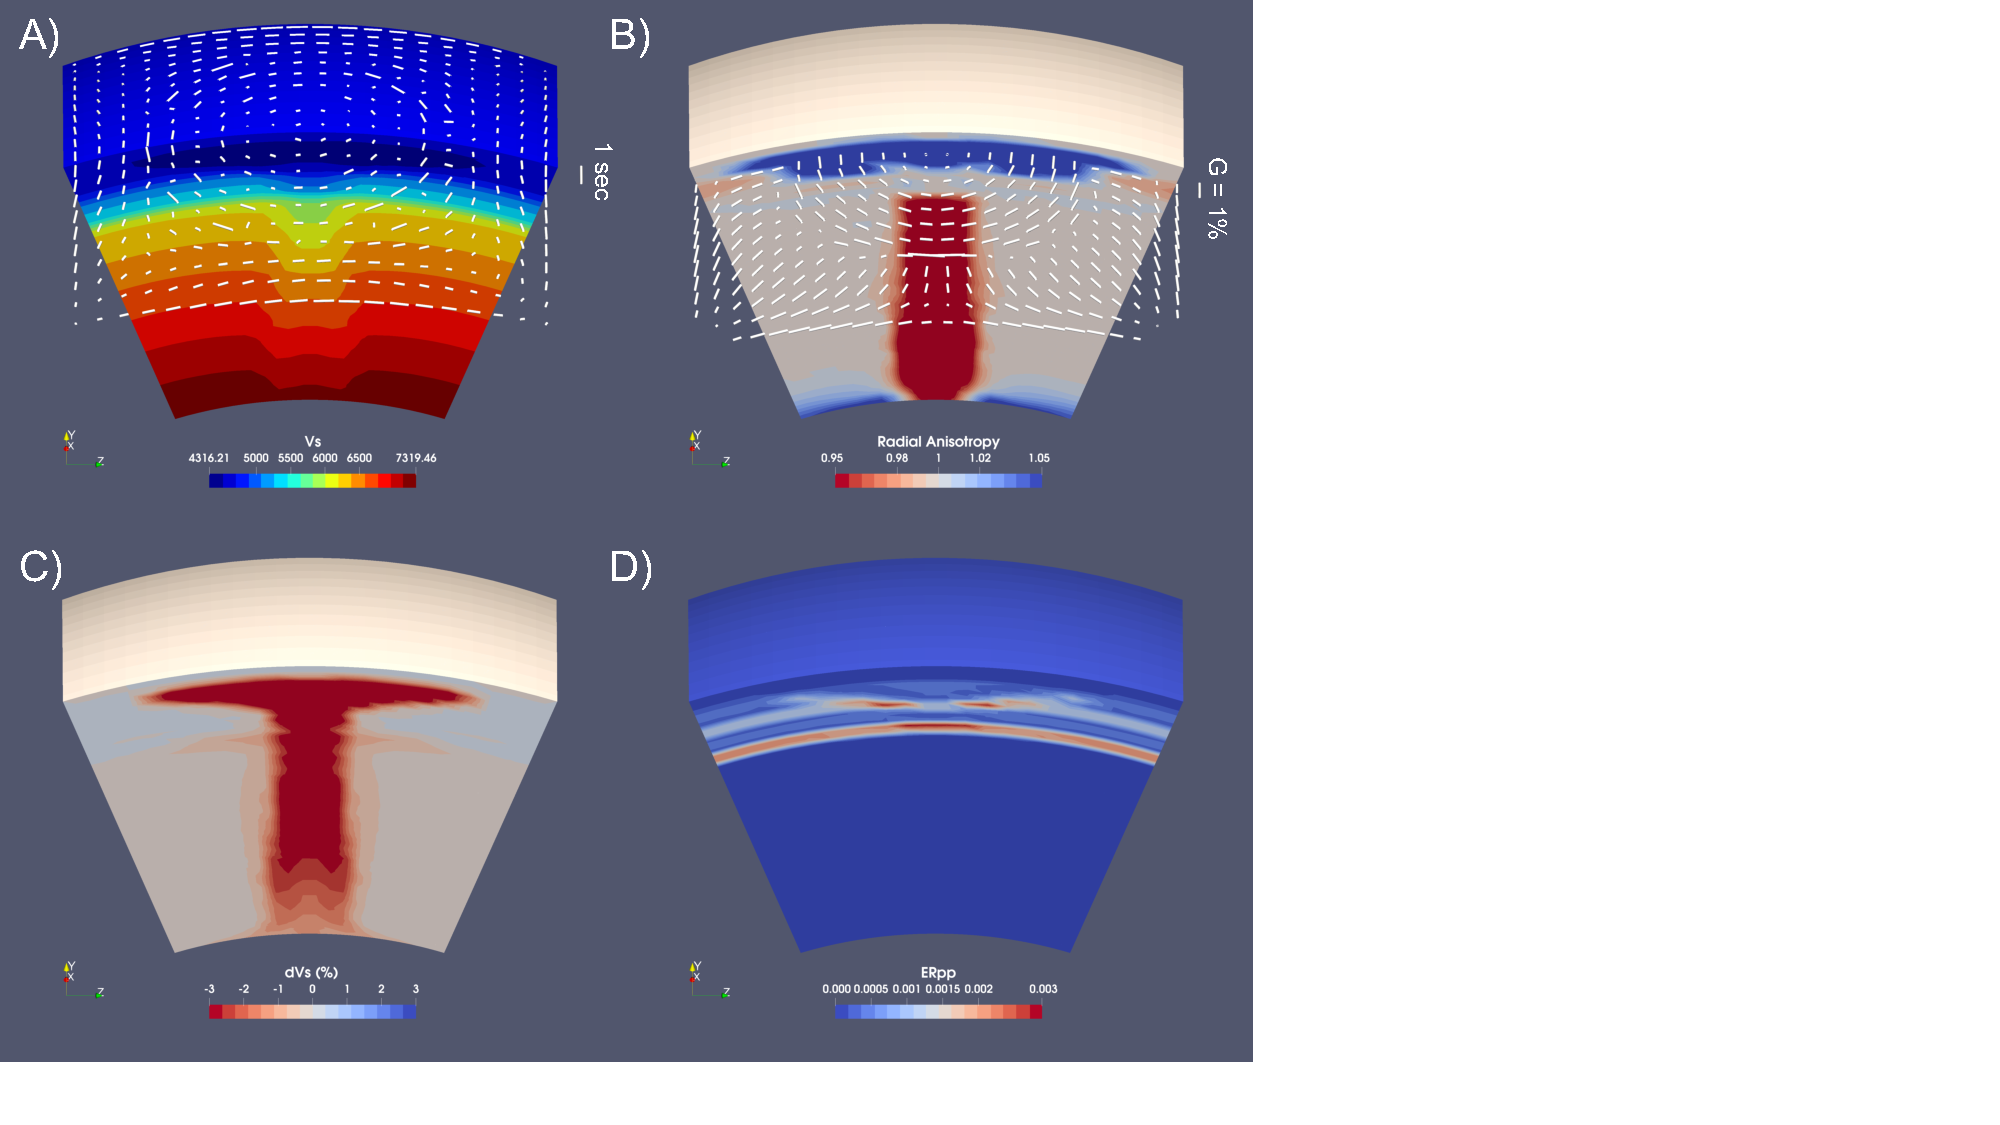
\includegraphics[width=1.0\textwidth]{VIZTOMO/plume.pdf}
    \caption{Example of a 3D thermo-mechanical model of an axi-symmetric thermal plume rising from the CMB in spherical coordinates. Only half of the eulerian grid generated with \viztomotitle{} is showed. A) S-wave isotropic velocity together with SKS splitting patterns at the surface (see chapter \ref{chapter:sks}); B) Radial anisotropy together with azimuthal anisotropy patterns (white bars) at 180 km depth; C) S-wave velocity anomalies (\%); D) Reflected P-P energy (note the lateral variations of the 410 and 660 km discontinuities as a function of the temperature anomaly).
    }
    \label{fig:plume}
\end{figure}

\begin{figure}[ht]
    \centering
    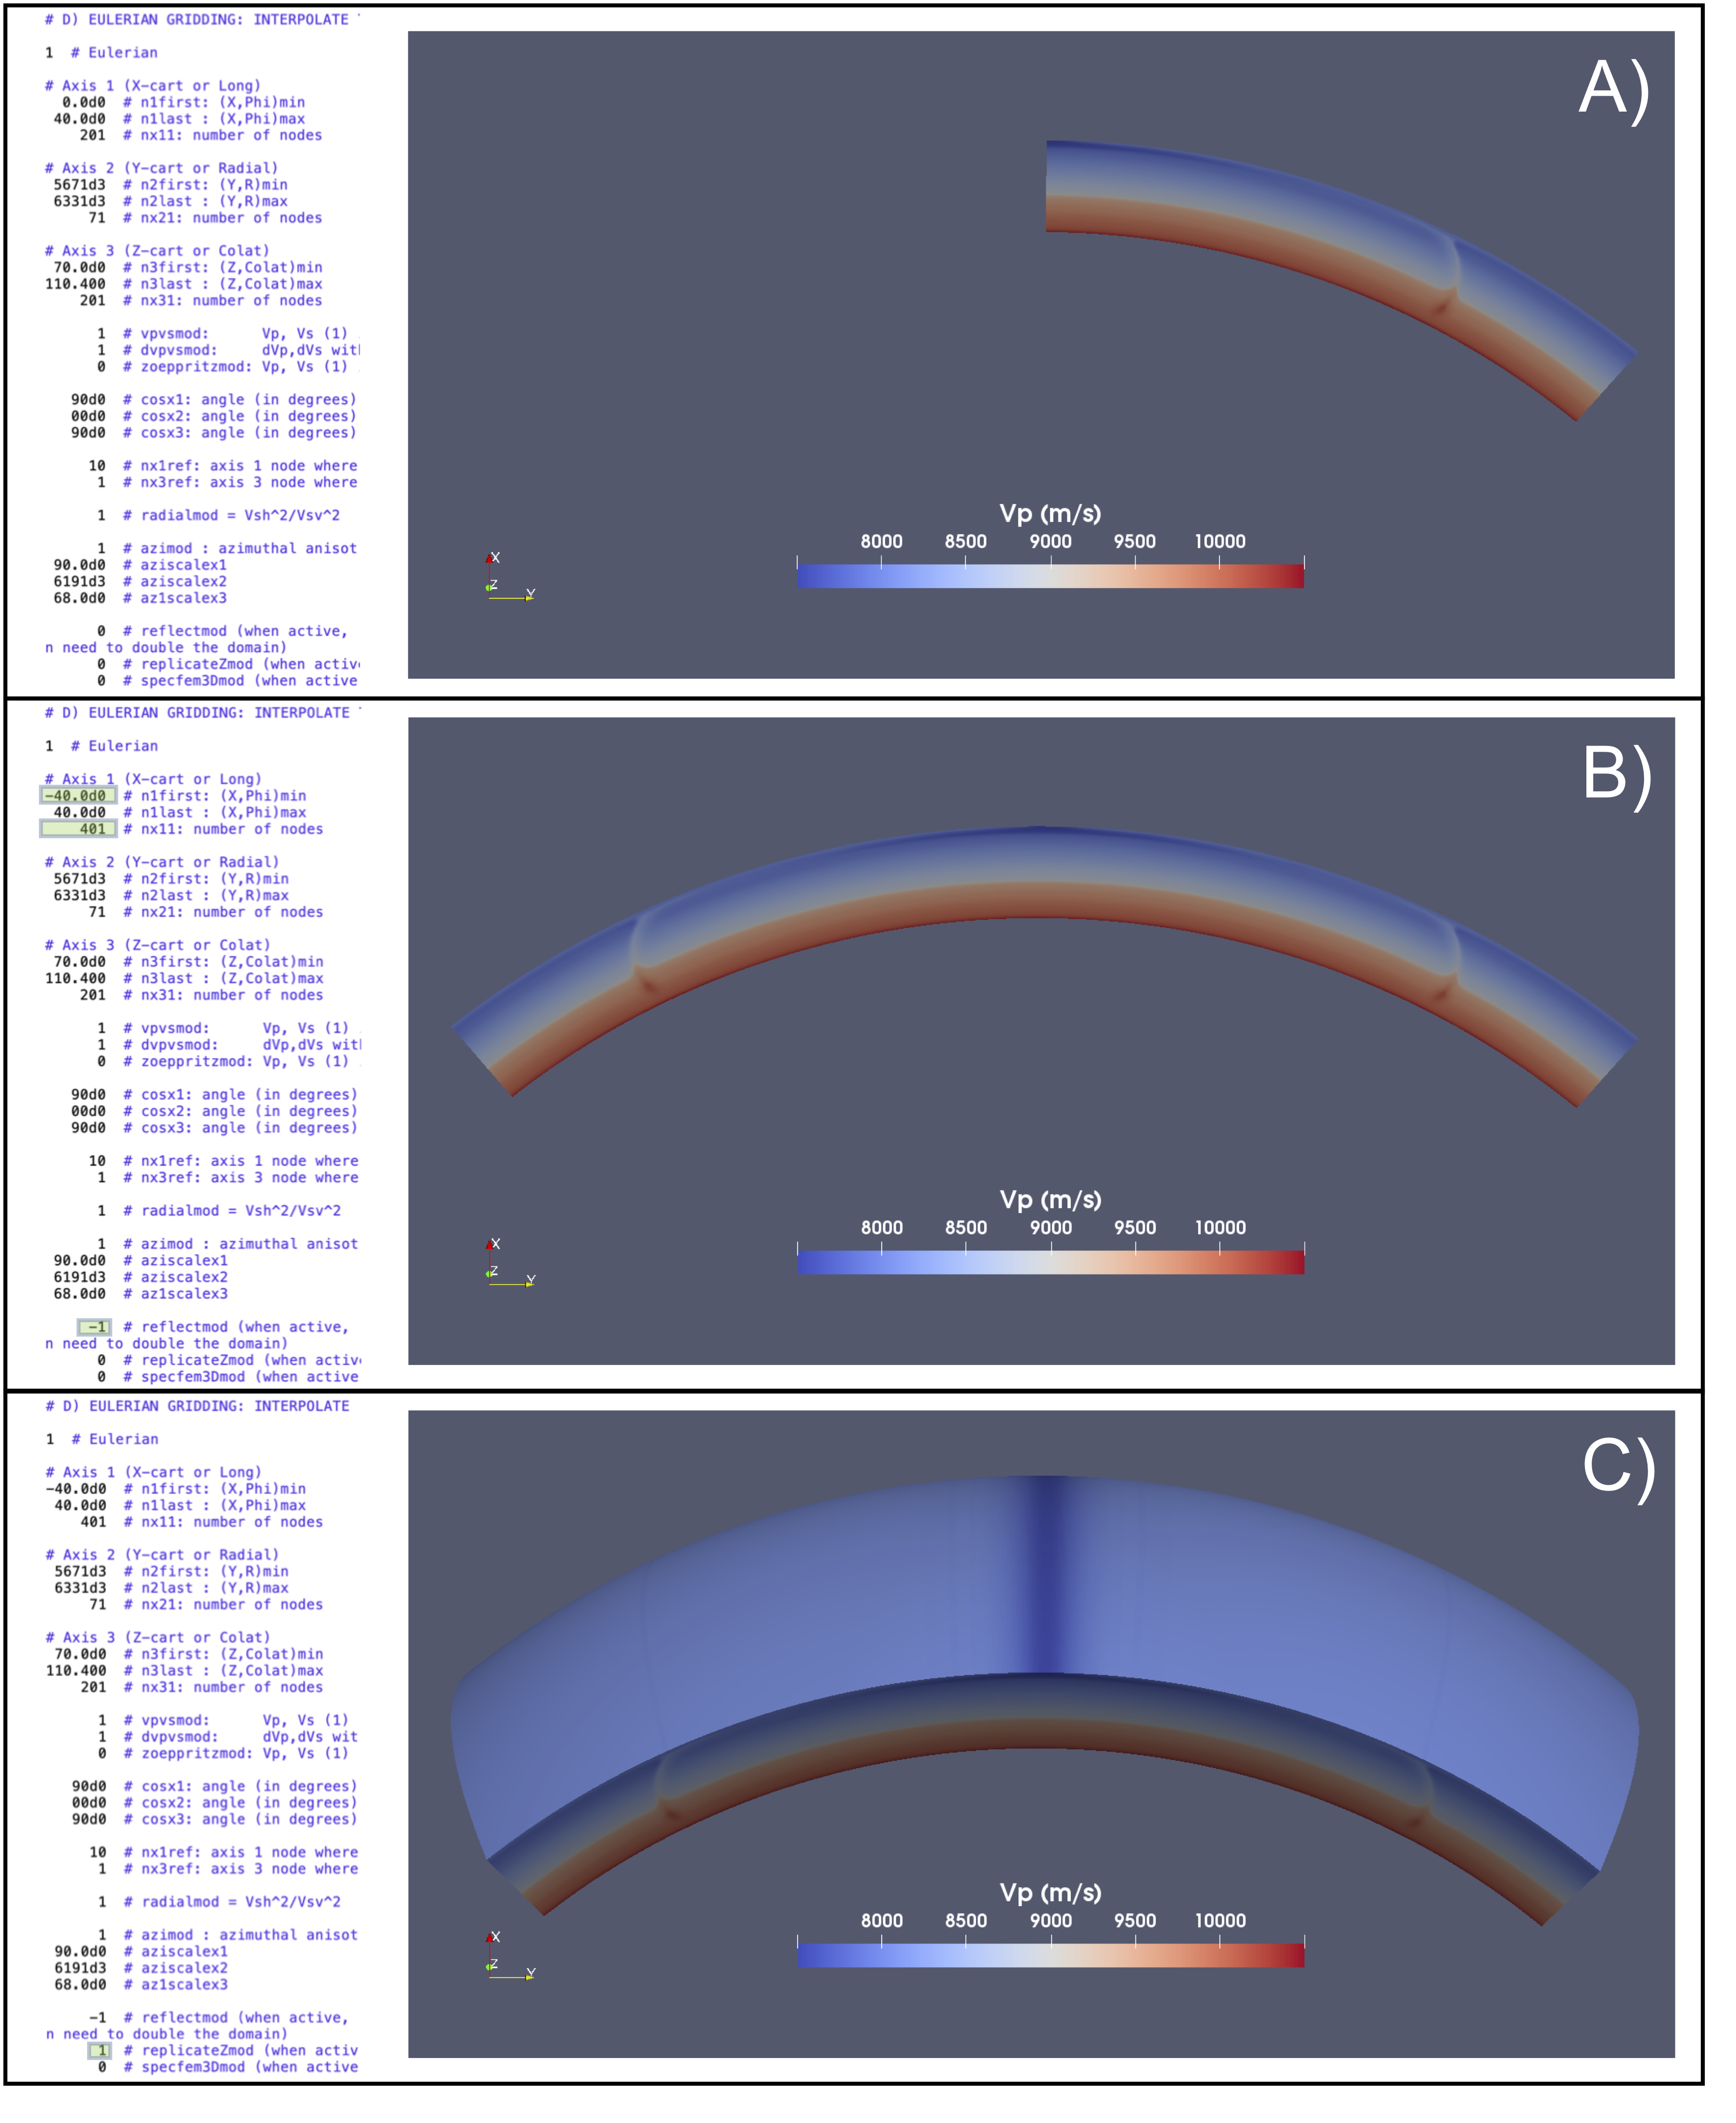
\includegraphics[width=1.0\textwidth]{VIZTOMO/reflectreplicate.png}
    \caption{Isotropic P-wave velocity of a 2D petrological-thermo-mechanical model of subduction in polar coordinates (see section \ref{section:cookbook_2Dsubduction}) (A). The same model reflected with respect to the oceanic ridge (B) and then replicated along the ridge axis (C). Right column: input variables in \texttt{viztomo\_input.dat}; the variations with respect to the configuration in the case right above is highlighted in pale green. Left column: P-wave velocity.  
    }
    \label{fig:reflectreplicate}
\end{figure}



%\vfill % Fill the rest of the page with whitespace


\section{SPECFEM3D simulations within the domain built with \viztomotitle{}}

To be finalized, coming soon!.\\

\vfill % Fill the rest of the page with whitespace